\documentclass[10pt,twocolumn,letterpaper]{article}

\usepackage{cvpr}
\usepackage{times}
\usepackage{epsfig}
\usepackage{graphicx}
\usepackage{amsmath}
\usepackage{amssymb}
\usepackage{booktabs}

% Include other packages here, before hyperref.

% If you comment hyperref and then uncomment it, you should delete
% egpaper.aux before re-running latex.  (Or just hit 'q' on the first latex
% run, let it finish, and you should be clear).
\usepackage[breaklinks=true,bookmarks=false]{hyperref}

\cvprfinalcopy % *** Uncomment this line for the final submission

\def\cvprPaperID{****} % *** Enter the CVPR Paper ID here
\def\httilde{\mbox{\tt\raisebox{-.5ex}{\symbol{126}}}}

% Pages are numbered in submission mode, and unnumbered in camera-ready
%\ifcvprfinal\pagestyle{empty}\fi
\setcounter{page}{1}
\begin{document}

%%%%%%%%% TITLE
\title{Truth or DeGPTion: Evaluating Lie Detection Capabilities of GPT-3.5 through Fine-Tuning on Personal Opinions, Autobiographical Memories, and Intentions}


\author{
Tanner Graves\\
{\tt\small tanneraaron.graves@studenti.unipd.it} \\
{\tt\small ID: 2073559} \\
\and
Marco Uderzo\\
{\tt\small marco.uderzo@studenti.unipd.it} \\
{\tt\small ID: 2096998} \\
\and
Francesco Vo \\
{\tt\small francesco.vo@studenti.unipd.it} \\
{\tt\small ID: 2079413} \\
\and
Mehran Faraji\\
{\tt\small mehran.faraji@studenti.unipd.it} \\
{\tt\small ID: 2071980} \\
\and
Claudio Palmeri \\
{\tt\small claudio.palmeri@studenti.unipd.it} \\
{\tt\small ID: 2062671} \\
}

\maketitle
%\thispagestyle{empty}


%%%%%%%%% ABSTRACT
\begin{abstract}
This paper aims at evaluating the capabilities of GPT3.5 in the task of Lie Detection.
This is done through the fine-tuning of GPT-3.5 on three English and Italian language datasets encompassing 
personal opinions, autobiographical memories, and future intentions. 
Fine-tuning of LLMs consists in adapting a pre-trained language model to a specific 
task by further training the model on task-specific data, thereby 
enhancing its ability to generate contextually relevant and coherent text in 
line with the desired task objectives. In our investigation, the objective is to 
discern and classify instances of truth or deception.

\end{abstract}

%%%%%%%%% BODY TEXT
\section{Introduction}
Numerous academic publications consistently prove that the human capacity to discriminate 
between veracity and deception rests at chance-level proficiency. Consequently, an escalating 
interest has emerged in the application of machine learning (ML) methodologies, particularly 
those leveraging the Transformer architecture, to enhance the accuracy of truthfulness prediction for statements. 
The intrinsic aptitude of ML models for pattern recognition empowers them to discern subtle cues 
that elude human perception. This paper employs OpenAI's GPT-3.5 Large Language Model (LLM) 
as the focal point, starting with an assessment of the base model's performance. Subsequently, 
an in-depth examination will be conducted on a fine-tuned GPT-3.5 model, specifically calibrated using the 
Personal Opinion Dataset (Deceptive Opinions), the Autobiographical Memories Dataset (Hippocorpus), and the 
Future Intentions Dataset, following \textit{'Scenario 3'} from Loconte et al.\cite{Loconte} \\

\subsection{Personal Opinion Dataset}

The participants of this study were divided in 4 groups (HIT’s) and asked to provide either 
a truthful or a deceptive opinion on the following topics: Abortion, Cannabis Legalization, Euthanasia, Gay Marriage, Policy on Migrants.
An extract from the table is shown below. \\

\begin{center}
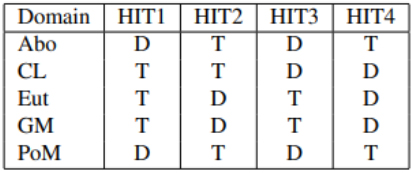
\includegraphics[scale=0.40]{img/pers_op_dataset.jpg} \\
\small {Example of the Personal Opinions Dataset.}
\end{center}

\begin{center}
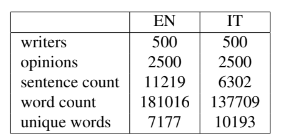
\includegraphics[scale=1]{img/dec_op_dataset_statistics.png} \\
\small {Descriptive Statistics of the Personal Opinions Dataset.} 
\end{center}

\subsection{Autobiographical Memories Dataset}

This dataset contains 6854 diary-like short stories about salient life events gathered in 3 steps from 2 groups of people (A,B).
The study was conducted as following:

\begin{itemize}
    \item Stage 1: Group A writes 15-25 sentence truthful stories with a 2-3 sentence summary and a timeframe
    \item Stage 2: Group B is tasked to write an imaginative story with the summary of group A as a prompt
    \item Stage 3: After 2 months group A is asked to retell the story starting with their summary as a prompt
\end{itemize}
At the end a questionnaire was posed. \\

\begin{center}
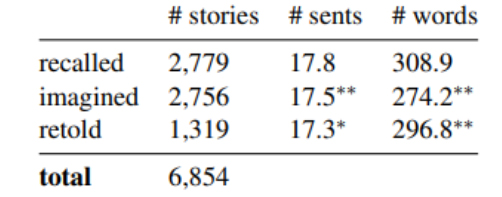
\includegraphics[scale=0.35]{img/autobio_mem_dataset.jpg} \\
\small {Descriptive Statistics of the Autobiographical Memories Dataset.}
\end{center}

\subsection{Future Intentions Dataset}

The Future Intentions Dataset is comprised of 1640 examples with two answer each, as each test subject had to answer 2 questions (Q1,Q2).
The study from which this dataset was collected was conducted as following.

All participants are divided into either the truthful or deceptful group.
The former were asked to describe a non-work-related activity that would be doing in the next seven days answering the following questions:

\begin{itemize}
    \item Q1: “Please describe your activity as specific as possible”
    \item Q2: “Which information can you give us to reassure us that you are telling the truth”
\end{itemize}

The latter were given 3 activities from the former group, asked which ones didn’t apply to them and get 
randomly assigned one of those. After, they were required to answer Q1, Q2 like the former group.
At the end a questionnaire was posed. \\

\begin{center}
    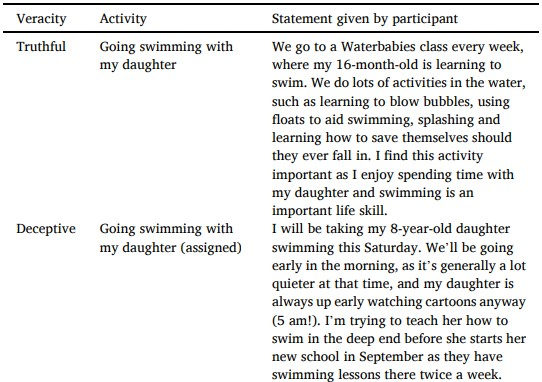
\includegraphics[scale=0.65]{img/future_intentions_dataset.jpg} \\
    \small {Example of the Future Intentions Dataset.} \\
\end{center} 


\begin{center}
    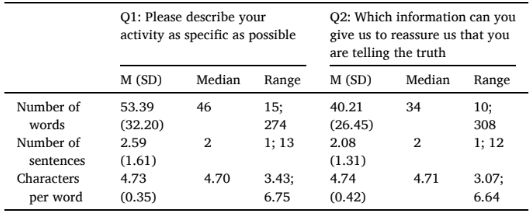
\includegraphics[scale=0.65]{img/future_intentions_dataset_statistics.png} \\
    \small {Descriptive Statistics of the Future Intentions Dataset.} 
\end{center}


\section{Methods}

\subsection{Dataset Preprocessing}

In our methodology, we adopted \textit{Scenario 3} as outlined by Loconte et al. \cite{Loconte}. 
This scenario involved the aggregation of three distinct train and test sets from \textit{Scenario 1}, 
which encompassed statements related to opinions, memories, and future intentions. Subsequently, 
the model underwent a fine-tuning process using the aggregated sets. 
The objective of \textit{Scenario 3} was to assess the model's overall capability to classify both truthful and deceptive 
statements across diverse contexts. Notably, in this scenario, the model was not fine-tuned to a specific type 
of statement; instead, it was evaluated on opinions, memories, and future intentions collectively, 
treating them as a randomly shuffled set of statements to be classified without bias towards any particular category. \\

The implementation of this process involved the merging of individual datasets into a unified one after cleaning and shuffling them.
The resulting dataset was then partitioned into training, validation, and test sets. It is essential 
to highlight that we intentionally did not utilize the entire initial dataset. The decision to employ a smaller 
training dataset was aimed to computationally simplify the training process of the LLM, while still ensuring effective learning and generalization. \\

As a final step, the datasets were formatted into \texttt{JSON} format to align with the expected input format of the OpenAI API, ensuring seamless integration with the API itself. 
For a detailed understanding of the implementation code, please refer to the \hyperref[sec:appendix]{Appendix} section of this paper, where the Python code is provided for reference.\\

Regarding the fine-tuning process, the two different models were trained using a smaller and bigger dataset as follows:

\begin{itemize}
    \item a subset of the original dataset (Train: 210 examples; Validation: 45 examples; Test: 45 examples).
    \item the full dataset (Train: 6765 examples; Validation: 1450 examples; Test: 1450 ??????? examples).
\end{itemize} \\

\subsection{GPT-3.5 Fine-Tuning}

This problem is a natural application for large language models, as the embeddings they learn in tandem
with their ability for self attention would seem a good model lie detection, and have shown promise with
similar problems. GPT-3.5 has been trained on an incredibly diverse dataset, and outperforms humans at lie
detection across all three datasets, despite not receiving specific training on this task. We aim to improve the
capability of GPT3.5 on the task through the process of fine tuning. OpenAI has maintained a high degree of
secrecy about their fine tuning process, not releasing the specifics of which parameters in the model
are tuned, or even how. The loss function employed is able to assess both differences between style and 
content between text, but in the case of a binary classifier loss is seen to loosely parody accuracy. 
In similarly large models, however, task specific fine-tuning will typically adjust parameters in the 
last couple layers before output. \\

In our study, we trained the model using the OpenAI API and evaluated its performance through testing 
and comparison with GPT-3.5. We also conducted additional experiments to understand how engineering 
the system prompt affects overall performance. One specific observation we made was regarding the baseline 
GPT-3.5's tendency to provide verbose or indecisive answers. When faced with statements that could be easily 
classified as genuine or deceptive, the model tended to provide detailed responses. However, in cases where 
it lacked sufficient information to confidently categorize a statement, the model often chose not to give a 
definitive answer.

To exemplify this behavior, let's consider the following scenario: when the model encounters uncertainty 
regarding a statement, it chooses not to offer a definitive classification. This characteristic underscores
the model's cautious approach when confronted with a potential lack of information, prioritizing the avoidance
of incorrect responses over providing answers that may be inaccurate.

\begin{verbatim}
User: "Each and every abortion 
is essentially a tragedy. The 
potential mother will suffer 
unforeseen consequences. Society
as a whole will be deprived of 
the potential it could have 
received from the new life."

   
Baseline GPT-3.5: "There is no 
objective truth to the statement 
as it expresses subjective opinions
and beliefs about abortion. It cannot 
be definitively classified as 
'True' or 'False'."
\end{verbatim}   

To mitigate this issue, we engineered a system prompt designed to 
discourage the verbose or indecisive behavior exhibited by the model. This tailored prompt also served
the crucial purpose of clearly conveying the task requirements to the model. Each time the model encountered 
an example query, it was presented with this prompt to guide its understanding and response.

Recognizing the importance of efficiency in both training and query costs, we took care to ensure that 
the instructions in the prompt were concise. The goal was to minimize any unnecessary token overhead that 
could contribute to an increased cost associated with training and queries.  \\

\begin{verbatim}
System Prompt to Fine-Tuned GPT-3.5:

"You are an expert capable of
discerning truthful from deceptive
opinions based on speech patterns. 
Definitively classify the following 
statement as 'True' or 'False', 
based on the likelihood the statement
represents a genuinely held belief 
or a deception."
\end{verbatim} \\

During the fine-tuning process, the model was incentivized to adopt the expected behavior and adhere to the specified output format. 
This reinforcement mechanism ensured that the model learned and internalized the desired characteristics, 
minimizing the likelihood of verbose or indecisive responses. \\

The hyperparameters used for fine-tuning the models are declared in 
the tables below, together with the fine-tuning training and validation losses over the steps.
It is important to clarify that the batch size - is the number of training examples used to train a single forward and backward pass - is not something under our control when fine-tuning.
By default, the batch size will be dynamically configured to be ~0.2\% of the number of examples in the training set.


\subsubsection*{300-Model Fine-Tuning}


\begin{center}

    \begin{tabular}{ccc}
        \toprule
        Hyperparameter & Value \\
        \midrule
        Learning Rate & ??? \\
        Epochs & ?? \\
        Batch Size & ?? \\
        \bottomrule
    \end{tabular}
\end{center} 

\begin{center}
    \small {Fine-Tuning Hyperparameters of the Cross-Validated model.} 
\end{center}

\begin{center}
\includegraphics*[scale=0.55]{img/training_loss_full.png} 
\end{center}

\begin{center}
    \small {Training Loss of the 300-Model (to change!).} 
\end{center}

\subsubsection*{Full-Model Fine-Tuning}

\begin{center}

    \begin{tabular}{ccc}
        \toprule
        Hyperparameter & Value \\
        \midrule
        Learning Rate & ??? \\
        Epochs & ?? \\
        Batch Size & ?? \\
        \bottomrule
    \end{tabular} 
\end{center} 

\begin{center}
    \small {Fine-Tuning Hyperparameters of the Full-Model.} 
\end{center}

\begin{center}
    \includegraphics*[scale=0.55]{img/training_loss_full.png} 
\end{center}

\begin{center}
    \small {Training Loss of the Full-Model.} 
\end{center}

\subsection{Cross-Validation}

Wanting to mitigate potential performance variation caused by the small test set of the 300-model, 
we implemented k-fold cross-validation for another set of models.
However, k-fold cross validation is a very resource-intensive process, and since we were using the official OpenAI API,
we were constrained by costs. Indeed, such validation becomes very expensive: GPT-3.5's pricing is \$0.0010 per 1,000 tokens 
for input and \$0.0020 per 1,000 tokens for output, where 1000 tokens equal about 750 words.
Because of the cost prohibitive nature of fine tuning large language models we would be training on 3 folds. 
Each of these folds will have 100 examples from each dataset sampled without replacement. 
This results in 3 models that were trained on 600 total examples and validated on a set of 300 examples. 
The OpenAI API uses the validation sets for hyperparameter selection, so a final test set is used to evaluate all models 
of 600 examples (200 from each set). The decision to give the classes equal representation in each fold was made as 
a consequence of previous models which underperformed on the Future Intentions Dataset and was
a minority class (16.6\% of training data for other models).

Below, the diagram explaining the cross-validation process is presented:

\begin{center}
\includegraphics*[scale=0.55]{img/cross_validation.png}
\end{center}

\begin{center}
    \small {Diagram of the Cross-Validation Process.} 
\end{center}

\begin{center}

    \begin{tabular}{ccc}
        \toprule
        Hyperparameter & Value \\
        \midrule
        Learning Rate & ??? \\
        Epochs & ?? \\
        Batch Size & ?? \\
        \bottomrule
    \end{tabular} 
 
\end{center}

\begin{center}
    \small {Fine-Tuning Hyperparameters of the Cross-Validated model.}
\end{center}

% CHANGE WITH ACTUAL ONE
\begin{center}
\includegraphics*[scale=0.55]{img/training_loss_full.png}
\end{center} 

\begin{center}
    \small {Training Loss of the Cross-Validated model.} 
\end{center}

\section{Results}

\subsection{Lie Detection Task Performance}

Initially, our evaluation began with the assessment of the non-fine-tuned
baseline GPT-3.5 model, resulting in an accuracy of 49\%, which is at chance level. Subsequently,
we fine-tuned two distinct models: the \texttt{300-Model} and the \texttt{Full-Model}, meaning
that the models were trained with 300 examples and the full training set respectively.
Upon completion of the fine-tuning process, we subjected both models to the same evaluation methodology. \\

As expected, the \texttt{300-Model} performed worse than the \texttt{Full-Model}. The latter exhibited a 
remarkable improvement in performance, achieving an overall accuracy of 82.2\%, whereas the former achieved an overall accuracy of 65.5\%.
This observation suggests that when fine-tuning, performance positively scales with the size
of the training set. Considering that the base GPT-3.5 model was performing at chance level, the fine-tuning process
yielded consistent and substantial enhancements in accuracy when it came to differenciating
between truthful and deceptive statements, even across multiple contexts. 
However, the aforementioned finding raises the problem of the trade-off between overall performance of the model
and training costs for fine-tuning when cross-validating. In fact, each OpenAI's API call is subject to a small fee, which, considering 
the total amount of calls needed and its positive relationship with the dimension of the training set, can result in great training costs.

In adherence to established Machine Learning best practices, the cross-validation approach allows for a comprehensive assessment 
of the model's generalization capabilities and robustness across diverse data samples, giving more accurate and reliable results. The choice of \texttt{k} 
is crucial for this process, and also determines the amount of resources that will be used. Ideally, 10-fold cross-validation is to be chosen.
Though, to keep the cost low, we decided to perform 3-fold cross validation on the \texttt{300-Model}. Considering this, it was expected that the cross-validated
smaller model would perform worse than the Full-Model, and we could safely assume that, without training costs as a factor, cross-validating the \texttt{Full-Model}
would have performed way better, closely to the non-cross-validated \texttt{Full-Model}.
The cross-validated \texttt{300-CV-Model} achieved 75.5\% accuracy (?), showing cross-validation to improve the performace over the \texttt{300-Model},
although, as expected, not being as accurate as the \texttt{Full-Model}.

The following table provides a detailed breakdown of the models' performances,
specifically focusing on accuracy:

\begin{center}

    \begin{tabular}{cc}
        \toprule
        Model & Overrall Accuracy \\
        \midrule
        Baseline GPT-3.5  & 49.5\% \\
        \midrule
        300-Model & 65.5\% \\
        \midrule
        Full-Model & 82.2\% \\
         \midrule
        300-CV-Model & 75.2\% \\
        \bottomrule
    \end{tabular}
    
\end{center}

\begin{center}
\small {Overall Accuracy of the models compared.}
\end{center}

\begin{center}

    \begin{tabular}{ccc}
        \toprule
        Model & Dataset & Accuracy \\
        \midrule
        Base GPT-3.5 & Personal Opinions & 49.5\% \\
                        & Autobio. Memories & 47.5\% \\
                        & Future Intentions & 51.5\% \\
        \midrule
        300-Model & Personal Opinions & 79.1\% \\
                    & Autobio. Memories & 67.3\% \\
                    & Future Intentions & 50.2\% \\
        \midrule
        Full-Model & Personal Opinions & 86.3\% \\
                    & Autobio. Memories & 82.3\% \\
                    & Future Intentions & 69.7\% \\
        \bottomrule
    \end{tabular} 
\end{center}


\begin{center}
    \small {Class-wise accuracy of the models compared.}
\end{center}

\begin{center}
    \begin{tabular}{lccc}
      \toprule
      & Model 1 & Model 2 & Model 3 \\
      \midrule
      Personal Op. & 83.5\% & 83.5\% & 80.0\% \\
      Autobio. Memories & 68.0\% & 69.5\% & 70.5\% \\
      Future Intentions & 72.5\% & 72.5\% & 70.0\% \\
      \midrule
      Macro avg. Acc. & 74.7\% & 75.2\% & 73.5\% \\
      \bottomrule
    \end{tabular}
\end{center}

\begin{center}
    \small {Class-wise accuracy of Cross-Validated model.}
\end{center}

\section{Discussion}

In the present study, we delved into the effectiveness of Large Language Models, specifically GPT-3.5, in the task of lie detection.
We considered both the baseline non-fine-tuned GPT-3.5 and two instances fine-tuned accordingly with \textit{'Scenario 3'} from Loconte et al.\cite{Loconte}. 
Our primary objective was to investigate the model's capacity to learn and generalize intrinsic linguistic representations of deception 
across a spectrum of contexts. This investigation was conducted using three distinct datasets, each comprising 
statements related to personal opinions, autobiographical experiences, and future intentions, thereby ensuring 
a comprehensive exploration of the model's capabilities. \\

Despite the baseline GPT-3.5 model's incapability to surpass human performance - where human capabilities 
typically hover around chance level - the fine-tuning process on the non-cross-validated \texttt{Full-Model} further enhanced its performance by 32.7\% in terms 
of accuracy.
This substantial improvement underscores the efficacy of the model to capture the nuances of deceptive language use.

Upon closer examination of performance by class, a noteworthy finding emerged: the models exhibited 
suboptimal performance on the Future Intentions Dataset, achieving a modest 69.7\% accuracy. 
This specific performance dip in one dataset had a discernible impact on the overall accuracy of the model. \\

When taking the \texttt{300-Model} into consideration, the overall accuracy gain compared to the baseline GPT-3.5 was 16\%. \\ 

Of particular interest was the observation that training GPT-3.5 on a smaller subset of data compromised
results when compared to training on a larger set. This observation has significant 
implications, making the fine-tuning process problematic in terms of training costs, 
expecially when following best practices like performing k-fold cross-validation. \\

The cross-validated \texttt{300-Model}, instead, represents the most accurate representation of the capability of the model trained
on the smaller dataset, improving its accuracy by an additional 9.7\%. \\

Future improvements on the project could be performing 10-fold cross-validation on the \texttt{Full-Model} to have a better understanding
of the full capabilities of GPT-3.5 in detecting deception leveraging the full dataset. Moreover, the use of stylometric analysis could shed
light on the linguistic styles of liars and how they differ from truth tellers.

\section{TO DO}

\begin{itemize}
    \item RAW DATA FILE!!
    \item training hyperparams (see table)
\end{itemize}

\section{Code Availability}
The datasets used and all the code used for this project is available
at the following \href{https://github.com/TannerAGraves/GPT-LieDetection/}{GitHub Repository}.


%-------------------------------------------------------------------------

{\small
\bibliographystyle{ieee_fullname}
\bibliography{egbib}
}

\clearpage % Start a new page
\onecolumn % Switch to one-column layout

\section{Appendix}
\label{sec:appendix}

We encourage to browse the Python Code directly from the GitHub repository at the following \href{https://github.com/TannerAGraves/GPT-LieDetection/}{link}.

\subsection{Python Code: Scenario 3 Dataset Preprocessing}

The following code preprocesses the dataset according to Scenario 3.
The original Python Notebook is located at the following \href{https://colab.research.google.com/github/TannerAGraves/GPT-LieDetection/blob/main/dataset/datasets.ipynb}{link} in our GitHub Repository

\begin{verbatim}
import numpy as np
import pandas as pd
from sklearn.model_selection import train_test_split

dc = pd.read_csv('DecOp_data_EN_500.csv', sep=',', encoding='UTF-8')

d1 = []
for i in range(dc.shape[0]):
  row = dc.iloc[i]
  d1.append({'ID': row['ID'],
      'age' :row['age'], 'gender': row['gender'],
  'sent' : row['A'].replace('\n', " ") ,
  'labels'  : row['GT.A']})

  d1.append({'ID': row['ID'],
      'age' :row['age'], 'gender': row['gender'],
  'sent' : row['E'].replace('\n', " ")  ,
  'labels'  : row['GT.E']})
  d1.append({'ID': row['ID'],
      'age' :row['age'], 'gender': row['gender'],
  'sent' : row['GM'].replace('\n', " ")  ,
  'labels'  : row['GT.GM']})

  d1.append({'ID': row['ID'],
      'age' :row['age'], 'gender': row['gender'],
  'sent' : row['Pom'].replace('\n', " ")  ,
  'labels'  : row['GT.Pom']})

  d1.append({'ID': row['ID'],
      'age' :row['age'], 'gender': row['gender'],
  'sent' : row['CL'].replace('\n', " ")  ,
  'labels'  : row['GT.CL']})

decop = pd.DataFrame.from_records(d1)

decop = decop[['ID', 'sent', 'labels']]
decop['type'] = 'A'

decop

hc = pd.read_csv('hcV3-stories.csv', sep=',', encoding='UTF-8')

mem = hc[hc['memType']!='retold']
mem = mem.dropna(subset=['story', 'memType'])
mem = mem[['story', 'memType']]
mem['memType'][mem['memType']=='recalled'] = 'T'
mem['memType'][mem['memType']=='imagined'] = 'F'
mem = mem.rename(columns={'story': 'sent', 'memType': 'labels'})
mem['type'] = 'B'

mem

intent = pd.read_csv('sign_events_data_statements.csv', encoding="UTF-8")

intent.loc[intent['outcome_class']=='t', 'outcome_class'] = 'T'
intent.loc[intent['outcome_class']=='d', 'outcome_class'] = 'F'
intent['q1'] = intent['q1'].apply(lambda x: x.replace('\n', ''))
intent = intent.rename(columns={'q1': 'sent', 'outcome_class': 'labels'})
intent = intent[['sent', 'labels']]
intent['type'] = 'C'

intent

k = 300
seed = 42

'''
shuffled_df = decop.sample(frac=0.1, random_state=seed).copy()
sample_decop = shuffled_df.iloc[:k,].copy()
sample_decop.drop('ID', axis=1, inplace=True)
sample_decop

data = pd.concat([sample_decop, mem.iloc[:k,].copy(), intent.iloc[:k,].copy()],
                 ignore_index=True)
'''

decop.drop('ID', axis=1, inplace=True)

data = pd.concat([decop, mem, intent], ignore_index=True)
data_shuffle = data.sample(frac=1, random_state=seed+27).reset_index(drop=True)
data_shuffle['labels'] = data_shuffle['labels'].map({'T': 1, 'F': 0})
data_shuffle.rename(columns={'sent': 'text', 'labels': 'label', 'type': 'set'}, 
                                                                        inplace=True)

data_shuffle = data_shuffle.iloc[:k,]

train_data, temp_data = train_test_split(data_shuffle, test_size=0.3, random_state=42)

val_data, test_data = train_test_split(temp_data, test_size=0.5, random_state=42)

train_data.to_json(f'train_data_{k}.json', orient='records', lines=True)

val_data.to_json(f'val_data_{k}.json', orient='records', lines=True)

test_data.to_json(f'test_data_{k}_class.json', orient='records', lines=True)

data_shuffle.shape

train_data.shape
\end{verbatim}

\subsection{Python Code: GPT-3 Fine-Tuning}

The following code fine-tunes GPT-3 using the official OpenAI APIs.
The original Python Notebook is located at the following \href{https://colab.research.google.com/github/TannerAGraves/GPT-LieDetection/blob/main/gpt3.5/API_scratch.ipynb}{link} in our GitHub Repository

\begin{verbatim}
import os
from openai import OpenAI
import pandas as pd
import json

key = os.environ.get("OPENAI_API_KEY")
client=OpenAI(api_key=key)

import json

def sanitize_to_utf8(input_str):
    """
    Sanitizes a string field to UTF-8.
    """
    return input_str.encode('utf-8', 'replace').decode('utf-8')

def process_jsonl_file(input_jsonl_path, output_jsonl_path):
    """
    Processes a JSONL file line by line, sanitizes each line to UTF-8,
    and saves it to a new JSONL file.
    """
    with open(input_jsonl_path, 'r', encoding='utf-8') as input_file, \
         open(output_jsonl_path, 'w', encoding='utf-8') as output_file:

        for line in input_file:
            # Parse JSON line
            json_obj = json.loads(line)

            # Sanitize data
            sanitized_json_obj = {key: sanitize_to_utf8(value) if isinstance(value, str) 
                                    else value for key, value in json_obj.items()}

            # Write sanitized JSON object to new JSONL file
            output_file.write(json.dumps(sanitized_json_obj) + '\n')

"""Generating intermediate 1500 example sets.

TODO: Preserve what dataset examples come from so we can breakdown performance by dataset.
"""

# Paths to your files
input_jsonl_path = 'train_data_full.json'
output_jsonl_path = 'output.jsonl'

# Process the JSONL file
process_jsonl_file(input_jsonl_path, output_jsonl_path)

sys_prompt = "You are an expert capable of discerning truthful from deceptive opinions 
                                                                based on speech patterns."

def gen_finetune(input, output, test=False):
    with open(input, 'r', encoding='utf-8') as data_in, \
        open(output, 'w') as gpt_out:
        for i, line in enumerate(data_in):
            user_prompt = json.loads(line)['text']
            sys_reply = "True" if json.loads(line)["label"] == 1 else "False"
            if not test:
                payload = {"messages": [{"role": "system", "content": sys_prompt}, 
                {"role": "user", "content": user_prompt}, {"role": "assistant", 
                                                            "content": sys_reply}]}
            else:# exclude response from test set
                payload = {"messages": [{"role": "system", "content": sys_prompt}, 
                {"role": "user", "content": user_prompt}]}
            gpt_out.write(json.dumps(payload) + '\n')

gen_finetune('train_data_300.json', 'train300_gpt.jsonl')
gen_finetune('val_data_300.json', 'val300_gpt.jsonl')

gen_finetune('train_data_1500.json', 'train1500_gpt.jsonl')
gen_finetune('val_data_1500.json', 'val1500_gpt.jsonl')

gen_finetune('train_data_full.json', 'train_full_gpt.jsonl')
gen_finetune('val_data_full.json', 'val_full_gpt.jsonl')

"""Example of querying model for classification.  
Example on model trained on 300 example set.
"""

test_lie = "One morning three months ago I was in a hurry and tripped on the steps 
while running to take a shower before work. I ended up fracturing 4 metatarsal bones 
that required two surgeries to fix. I was really having a hard time not being able 
to walk whenever I wanted to. I really had such a bad attitude at the beginning 
because I was so used to being independent. Now that I have recovered I have a 
new appreciation for my ability to walk. I feel like the whole time I couldn't 
walk I was thinking about how much I took that ability for granted. But now I 
choose to walk more than I ever had before. When I walk the dogs I go further 
out of my way just to enjoy the ability to do it. I am completely recovered 
and I am going to take this as a lesson learned. Nothing is more important 
that my personal health. I need to make sure that even if I am running late, 
I need to take my time and be careful. Instead f making it to work on time, 
I ended up missing weeks of work. Now all I do at work is try and catch up 
with everything I missed. It was really nice that people at work came and 
visited me at the hospital. I really appreciated all the flowers and candy 
and food that was delivered. I think that this showed me how loved I truly am."

test_truth = "Each and every abortion is essentially a tragedy. 
The potential mother will suffer unforeseen consequences. Society as a whole will 
be deprived of the potential it could have received from the new life."

response = client.chat.completions.create(
  model="ft:gpt-3.5-turbo-0613:personal::8S542QSs",
  messages=[
    {"role": "system", "content": sys_prompt},
    {"role": "user", "content": test_lie},
    {"role": "user", "content": test_truth},
  ]
)
response.choices[0].message.content

mdls = {
    '300':"ft:gpt-3.5-turbo-0613:personal::8S542QSs",
    '3.5':"gpt-3.5-turbo",
    '1500':"ft:gpt-3.5-turbo-0613:personal::8TAkdwiX"
    }

def predict(text, model, sys_prompt):
    response = client.chat.completions.create(
    model=model,
    messages=[
        {"role": "system", "content": sys_prompt},
        {"role": "user", "content": text}
    ]
    )
    return response.choices[0].message.content

test_truth

test_lie

def eval(test_file, mdl, return_df = False, sys_prompt=sys_prompt, by_class=False):
    msgs = []
    preds = []
    trues = []
    replies = []
    set = []
    with open(test_file, 'r') as f:
        for ex in f:
            ex = json.loads(ex)
            msg = ex['text']
            #pred = predict(msg, mdl) == 'True' #'True' if predict(msg) else 'False'
            reply = predict(msg, mdl, sys_prompt) #for debug
            pred = reply == 'True'
            true = ex['label'] == 1
            msgs.append(msg)
            preds.append(pred)
            trues.append(true)
            replies.append(reply) # debug
            if by_class:
                set.append(ex['set'])
    if by_class:
         test_df = pd.DataFrame.from_dict({'msg': msgs, 'reply':replies, 
                            'preds': preds, 'target': trues, 'set':set})
    else:
        test_df = pd.DataFrame.from_dict({'msg': msgs, 'reply':replies, 
                            'preds': preds, 'target': trues})
    acc = (test_df['preds'] == test_df['target']).mean()
    if return_df:
        return (test_df, acc)
    else:
        return acc


test_truth

sys_prompt_base = sys_prompt + ' Definitively classify the following statement 
                as \'True\' or \'False\', based on the likelihood  the statement 
                represents a genuinely held beleif or a deception.'
#base_df, base_acc = predict('test_data_300.json', mdls['3.5'])
predict(test_truth, mdls['300'], sys_prompt=sys_prompt)

test300_df, test300_acc = eval('test_data_300.json', mdls['300'], True, 
                                                            sys_prompt=sys_prompt)
print(test300_acc)
test300_df

test300_acc

test35_df, test35_acc = eval('test_data_300.json', mdls['3.5'], True, 
                                                        sys_prompt=sys_prompt_base)
print(test35_acc)
test35_df

len(test1500_df)

# Takes a lot of time, cost = $1
#test1500_df, test1500_acc = eval('test_data_1500.json',mdls['1500'],True,
                                                            sys_prompt=sys_prompt)
print(test1500_acc)
test1500_df

test1500_df.to_csv('results1500.csv')

"""Model / Dataset Bias analysis:"""

print('Model truth classification rate: ')
print(test300_df['preds'].mean())
print('Dataset truthful statement rate: ')
print(test300_df['true'].mean())

"""Model performance by dataset"""

sys_prompt

class_df, class_acc = eval('test_data_1500.json', mdl=mdls['1500'], 
                            sys_prompt=sys_prompt, return_df=True, by_class=True)

class_df['correct'] = class_df['preds'] == class_df['target']
class_df.groupby('set')['correct'].mean()

class_df.to_csv('results_class.csv')
\end{verbatim}




\end{document}
